\documentclass{svproc}

\usepackage{url}
\usepackage{hyperref}
%\usepackage{hypernat}
\usepackage{cite}
%\usepackage[numbers,compress]{natbib}

\usepackage{adjustbox}
\usepackage{amsmath}
\usepackage{amssymb}
\usepackage{color,soul}

\begin{document}

\title{Parallel Computations for Solving Multicriteria Mixed-Integer Optimization Problems}

\author{Victor Gergel \and Evgeniy Kozinov}

\institute{Institute of Informational Technologies, Mathematics and Mechanics, Mathematical Center, Lobachevsky State University of Nizhny Novgorod, Nizhni Novgorod, Russia \\
\email{gergel@unn.ru, evgeny.kozinov@itmm.unn.ru}
}

\maketitle              % typeset the title of the contribution


\begin{abstract}
The paper discusses a new approach to solving computationally time-consuming multicriteria optimization problems, in which some variable parameters can only take on discrete values. Under the proposed approach, the solution of mixed-integer optimization problems is reduced to solving a family of optimization problems where only continuous parameters are used. All problems of the family are solved simultaneously in the time division mode, where the optimization problem for the next global search iteration is selected adaptively taking into account the search information obtained in the course of the calculations. The algorithms proposed enable parallel computing on high-performance computing systems. Computational experiments confirm that the proposed approach makes it possible to significantly reduce computation volume and time for solving complex multicriteria mixed-integer optimization problems.
\keywords{Multicriteria optimization $\cdot$ multi-integer optimization problems $\cdot$ methods of criteria scalarization $\cdot$ global optimization $\cdot$ search information $\cdot$ parallel computing $\cdot$ computational experiment}
\end{abstract}


\section{Introduction}\label{sec:1}

Multicriteria optimization (MCO) problems arise almost every time when the best options need to be chosen when developing complex technical facilities and systems. The scale of demand for MCO problems determines the high intensity of research in this area -- see, for example, monographs \cite{c1,c2,c3,c4,c5} and reviews of scientific and practical results in this area \cite{c6,c7,c8,c9}.

Usually, the solution of a MCO problem is a set of efficient (non-dominated) decisions for which an improvement in values with respect to some criteria cannot be achieved without deteriorating the efficiency with respect to some other criteria. The definition of the whole set of efficient decisions (the Pareto set), on the one hand, may require a large amount of computation and, on the other hand, may be redundant as the analysis of a large number of efficient decisions may require a significant effort for the person who makes the decision (decision maker, DM). Thus, it may be practically justified to find only a relatively small set of efficient decisions that can be formed according to the optimality requirements defined by the DM. 

By limiting the set of efficient decisions to be computed, one can achieve a noticeable reduction in the amount of calculations required. However, efficiency criteria may be complex, \textit{multi-extremal}, and calculating the values of these criteria can prove \textit{computationally demanding}. In addition, some variables may only take on discrete values. In such cases, MCO problems involve \textbf{significant computational complexity}, which can only be overcome by using high-performance supercomputer systems.

Many different approaches have been proposed for solving MCO problems (see, for example, \cite{c3,c6,c10,c11}.  Most commonly, various methods based on reduction of the vector criterion to a particular scalar function are used \cite{c2,c12}. The number of works on multicriteria mixed-integer problems is however more limited -- in most cases, the issues of discrete parameter analysis are considered in relation to scalar optimization problems (see, for example, reviews \cite{c13,c14}). The widely used deterministic methods for solving problems of this class are usually based on the Branch-and-Bound \cite{c15} or on the Branch-and-Reduce approaches \cite{c16}. A number of meta-heuristic and genetic algorithms are also known and are based, in one way or another, on the random search concept \cite{c17,c18}.

This paper presents the results of research that was carried out to develop highly effective parallel methods of multicriteria optimization making use of all the search information obtained in the course of calculations \cite{c19,c20,c21}. A new contribution to this research area consists in the development of an approach for solving MCO problems, in which some of the variable parameters can only take discrete values. The proposed approach reduces the solution of mixed-integer optimization problems to a family of optimization problems where only continuous parameters are used. All problems of the family are solved simultaneously in the time division mode, where the selection of the optimization problem for the next iteration of the global search is performed adaptively taking into account the search information obtained in the course of the calculations. The algorithms developed enable efficient parallel computing on high-performance computing systems.

The rest of the paper is organized as follows. In Section \ref{sec:2}, we give the statement of multicriteria optimization problems, present a minimax scheme for scalarization of the vector efficiency criterion and introduce the concept of multistage solution of multicriteria optimization problems. In Section \ref{sec:3}, we present a description of the proposed approach based on the reduction of mixed-integer optimization problems to solving a family of optimization problems with the use of only continuous parameters. This section also describes a dimensionality reduction scheme, which allows multidimensional optimization problems to be reduced to a one-dimensional global search problem. Section \ref{sec:4} presents a parallel algorithm for solving multicriteria multi-integer optimization problems, which is used in the framework of the proposed approach. Section \ref{sec:5} contains the results of numerical experiments confirming that the proposed approach is quite promising. In conclusion, the results obtained are discussed and possible main directions for continuing the research are outlined.


\section{Problems of Multicriteria Mixed-Integer Optimization}\label{sec:2}

The problem of multicriteria mixed-integer optimization (MCOmix) can be formulated as follows
\begin{equation}\label{eq:1}
f(y,u)\to \min, y\in D,u \in U,
\end{equation}
where $f(y,u)=(f_1 (y,u),f_2 (y,u), \dots,f_s (y,u))$ is the vector criterion of efficiency in which the variable parameters belong to two different types:
\begin{itemize}
	\item continuous parameters $y=(y_1,y_2,\dots,y_n)$, whose domain of possible values is represented by an $N$-dimensional hyperparallelepiped:
\begin{equation}\label{eq:2}
D=\{ y\in R^n: a_i \leq y_i \leq b_i, 1 \leq i \leq n \}, 
\end{equation}
for specified vectors $a$ and $b$.
	\item discrete parameters  $u=(u_1,u_2, \dots ,u_m)$, each of which can only take on a fixed (discrete) set of values:
\begin{equation}\label{eq:3}
U=U_1 \times U_2 \times \dots \times U_m=\{w_k=<w_{1k},w_{2k}, \dots, w_{mk}>: 1 \leq k \leq l\}, w_{ik} \in U_i, 
\end{equation}
where $U_i=\{v_{i1},v_{i2}, \dots ,v_{il_i} \}$, $1 \leq i \leq m$, is a set of $l_i>0$ admissible discrete values for the parameter $u_k$, i.e., the whole set of all possible discrete parameter values $U$ contains
\begin{equation}\label{eq:4}
  l=\prod\limits^m_{i = 1}{l_i}
\end{equation}
different elements (tuples $w_k$,$1 \leq k \leq l$). Without loss of generality, it will be assumed in further consideration that the criteria $f_i (y,u)$, $1 \leq i \leq s$, are non-negative and their reduction corresponds to an increase in the efficiency of the decisions selected.
\end{itemize}

In the most complex variant, the criteria $f_i(y,u)$, $1 \leq i \leq s$, may be multi-extremal, and the procedures for calculating their values can be computationally time-consuming.  It is also assumed that the criteria $f_i (y,u)$, $1 \leq i \leq s$, meet the Lipschitz condition   
\begin{equation}\label{eq:5}
  |f_i (y_1,u_1 )-f_i (y_2, u_2 )| \leq L_i \|(y_1, u_1)-(y_2, u_2)\|, 1 \leq i \leq s,
\end{equation}
where $L_i$ is the Lipschitz constant for the criterion $f_i (y,u)$, $1 \leq i \leq s$,  and $\|*\|$ denotes the Euclidean norm in $R^N$. 

Efficiency criteria in an MCO problem are usually controversial and the parameters $(y^*,u^*) \in D \times U$ with the best values for all criteria at the same time may not be available. In such situations, it is a common approach for MCO problems to find efficient (non-dominated) decisions, for which an improvement in the values of some criteria leads to a deterioration of efficiency indicators for other criteria. Obtaining the whole set of efficient decisions (the Pareto set) can require a lot of computation and, as a result, another approach is often used -- to find only a relatively small set of efficient decisions defined according to the decision maker's requirements.

A commonly used approach to obtaining individual efficient decisions is to transform a vector criterion into some common scalar efficiency index\footnote{It should be noted that this approach ensures that a wide range of already existing global optimization methods can be used to solve MCO problems.}
\begin{equation}\label{eq:6}
  \min{F(\alpha,y,u)}, y \in D, u \in U,
\end{equation}
where $F$ is an objective function generated by scalarization of the criteria $f_i$, $1 \leq i \leq s$, $\alpha$ is the vector of the parameters of the criteria convolution applied, while $D$ and $U$ are the domains of possible parameter values from (\ref{eq:2}-\ref{eq:3}). By virtue of (\ref{eq:5}), the function $F(\alpha, y, u)$ also satisfies the Lipschitz condition with some constant $L$, i.e.  
\begin{equation}\label{eq:7}
  |F(\alpha, y_1, u_1)-F(\alpha, y_2, u_2)| \leq L\|(y_1,u_1)-(y_2,u_2)\|.
\end{equation}

To construct a common scalar efficiency index $F(\alpha,y,u)$ from (\ref{eq:6}), one of the most frequently used scalarization methods is to use a minimax criteria convolution \cite{c2,c5}:
\begin{equation}\label{eq:8}
\begin{matrix}
  F(\lambda,y,u)=\max{(\lambda_i f_i (y,u),1\leq i \leq s)},\\
  \lambda=(\lambda_1,\lambda_2, \dots, \lambda_s)\in \Lambda \subset R^s: \sum_{i=1}^{s}\lambda_i=1, \lambda_i \geq 0, 1 \leq i \leq s.
\end{matrix}
\end{equation}

It should be noted that due to the possible changes in the requirements for optimality in the process of calculations it may be necessary to change the parameters of the convolution $\lambda$ from (\ref{eq:8}). Such variations yield a set of scalar global optimization problems (\ref{eq:6})
\begin{equation}\label{eq:10}
\mathbb{F}_T=\{F(\alpha_t,y):1 \leq t \leq T\},
\end{equation}
which is necessary for solving the MCOmix problem. This set of problems can be formed sequentially in the course of calculations; the problems of the set can be solved strictly sequentially or simultaneously in time division mode. In addition, the problems of the set $\mathbb{F}_T$ can be solved in parallel using high-performance computing systems. The possibility of forming the set $\mathbb{F}_T$ defines a \textit{new approach to multistage solution of multicriteria optimization} (MMCO) problems -- see, for example, \cite{c22}.


\section{The Approach: Unrolling Mixed-Integer Optimization Problems and Dimensionality Reduction}\label{sec:3}

In the presence of discrete parameters, solving multicriteria optimization  problems becomes considerably  more complicated -- in many cases, it becomes necessary to calculate criterion values for all possible values of discrete parameters. The proposed approach to improving the efficiency of solving MCOmix problems is based on the following two basic ideas: unrolling mixed-integer optimization problems \cite{c23} and dimensionality reduction \cite{c24,c25}.

\subsection{Simultaneous Solution of Mixed-Integer Optimization Problems} \label{subsec:31}

To solve the global optimization problem (\ref{eq:6}), a two-stage nested optimization scheme can be used
\begin{equation}\label{eq:11}
\begin{matrix}
  F(\alpha,y^*,u^*)=\min{F(\alpha,y,u)} \min_{y \in D} \min_{u \in U}{F(\alpha,y,u)} =\\ 
  \min_{y \in D}(F(\alpha,y,w_1 ),F(\alpha,y,w_2 ), \dots, F(\alpha,y,w_l )),w_i\in U,1 \leq i \leq l.
\end{matrix}
\end{equation}

In the computational scheme (\ref{eq:11}), for any value of continuous parameters $y \in D$, the values of the function $F(\alpha,y,u)$ are calculated for all possible values of discrete parameters $u \in U$. However, the smallest value of the function $F(\alpha,y,u)$ is achieved only with one specific value of discrete parameters $u^*$, so the calculation of function $F(\alpha,y,u)$ values for other values of discrete parameters is redundant. Thus, for example, for the problem
\begin{equation}\label{eq:12}
 \min\{u^2(sin(x)+sin(10x/3)):x\in[2.7,7.5],u\in \{1,2\}\}
\end{equation}
having one continuous and one discrete parameter, the plots of the  function $F(\alpha,y,u)$ for different values of the discrete parameter have \hl{form from }Fig.~\ref{fig:1} 
\begin{figure}
  \centering
  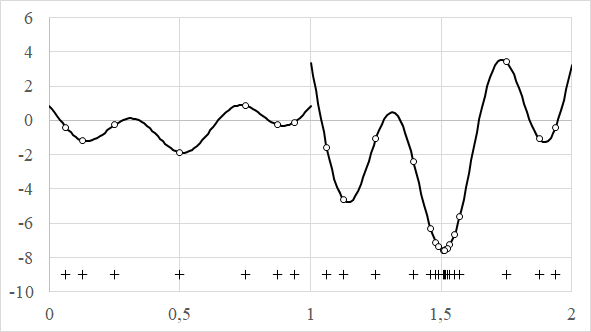
\includegraphics[width=0.9\linewidth]{fig1}
  \caption{The function $F(\alpha,y,u)$ of the problem (\ref{eq:12}) plotted for different values of the discrete parameter (left, $u=1$,  right, $u=1$)}
  \label{fig:1}
\end{figure}
and, as one can see, there is no need to calculate the value of the function $F(\alpha,y,u)$ for $u=1$.

It is possible to increase the efficiency and, accordingly, to reduce computational complexity when solving  the problem (\ref{eq:6}) by excluding (or at least by reducing) the calculation of the function $F(\alpha,y,u)$ for discrete parameters $u \neq u^*$. In some rare situations, the information about the values of the discrete parameters that do not allow the minimum value of the function $F(\alpha,y,u)$ to be reached, may be known a priori. In most cases, such information can be obtained only in the process of calculations based on the obtained search information. 

Assume that 
\begin{equation}\label{eq:13}
 \omega_k=\{ y^i,u^i,z^i=F(\alpha,y^i,u^i ): 1\leq i\leq k \}
\end{equation}
is the search information obtained in the process of calculation after global search iterations. Then the procedure for adaptive estimation of the discrete parameter value, at which the minimum value  of the function $F(\alpha,y,u)$ is expected to be obtained, can be determined using the decision rule
\begin{equation}\label{eq:14}
	\theta =\Theta(\omega_k ),1 \leq \theta \leq l, 
\end{equation}
 that determines the most promising value of the discrete parameter $u \in U$ at each step of the global search.

With the decision rule $\Theta$, the general computational scheme for solving the problem can be presented as follows.

\textit{Rule 1.} Apply the decision rule $\Theta$ from (\ref{eq:14}) to available search information $\omega_k$ from (\ref{eq:13}),  and determine the value of the discrete parameter $u=w_\theta$, $w_\theta \in U$.
 .
\textit{Rule 2.} Determine the point $y \in D$ of the global search iteration to be performed with a fixed value of the discrete parameter $u=w_\theta$, $w_\theta \in U$.
			
\textit{Rule 3.} Check the stopping condition for the computation. If the required accuracy of the global search is not achieved, it is necessary to supplement the search information $\omega_k$ from (\ref{eq:13}) with the results of the current iteration and execute rule 1.

   The above computational scheme will be presented in more detail after the description of the global search algorithm. 



\subsection{Dimensionality Reduction of Mixed-Integer Optimization Problems} \label{subsec:32}

It should be noted that the computational complexity of solving global optimization problems increases exponentially with increasing dimensionality. The problem of increasing computational complexity was even called the ``dimensionality curse''. In particular, when applying the computational scheme discussed in paragraph \ref{subsec:31}, it is necessary to accumulate and analyze multidimensional search information $\omega_k$ from (\ref{eq:13}). This computational complexity can be significantly reduced by reducing the optimization problems to be solved by using Peano \textit{curves} or \textit{evolvents} $y(x)$, which unmbiguously and continuously map a segment [0,1] on an $n$-dimensional hyper-cube $D$ -- see, for example, \cite{c24,c25}. As a result of this reduction, the multidimensional global optimization problem (\ref{eq:6}) is reduced to a one-dimensional problem:
\begin{equation}\label{eq:15}
 \min_{y\in D, u \in U}F(\alpha,y,u) = \min_{x \in [0,1]}(F(\alpha,y(x),w_1 ),F(\alpha,y(x),w_2 ),\dots,F(\alpha,y(x),w_l ))
\end{equation}

It should be noted that the one-dimensional functions $F(\alpha,y(x),u)$ resulting from the reduction, with a fixed value of discrete parameters $u \in U$ satisfy the uniform H{\" o}lder condition, i.e.
\begin{equation}\label{eq:16}
|F(\alpha, y(x_1),u_1)-F(\alpha, y(x_2),u_2)| \leq H|x_1-x_2 |^{1/n},
\end{equation}
where the constant $H$ is determined by the relation $H=2L\sqrt{N+3}$, $L$ is the Lipschitz constant from (\ref{eq:7}) and $n$ is the dimensionality of the optimization problem (\ref{eq:1}). 

As a result of dimensionality reduction, the search information $\omega_k$ from (\ref{eq:13}) obtained in the calculation can be presented in the form 
\begin{equation}\label{eq:17}
A_k=\{(x_i, u_i, z_i, f_i = f(y(x_i), u_i): 1 \leq i \leq k \},
\end{equation}
where $x_i$, $u_i$, $1 \leq i \leq k$,  are the points of the global search iterations, $z_i$, $f_i$, $1 \leq i \leq k$,  are the values of the scalar criterion $F(\alpha,y(x),u)$ and the criteria $f_i (y)$, $1 \leq i \leq s$, calculated at the points $x_i$, $u_i$, $1 \leq i \leq k$. Note that the data in the set $A_k$ are arranged in ascending order\footnote{Data ordering is reflected by using a subscript.} of the points $x_i$, $1 \leq i \leq k$, i.e.
\begin{equation}\label{eq:18}
 x_1< x_2< \dots < x_k
\end{equation}
for a more efficient execution of global search algorithms.

The use of dimensionality reduction makes it possible to combine (concatenate) one-dimensional functions into a single one-dimensional function $\Phi(\alpha,y(x))$, defined over the segment $[0,l]$ (see Fig.~\ref{fig:1}).

\begin{equation}\label{eq:19}
 \Phi(\alpha,y(x)) = 
\begin{cases}
F(\alpha,y(x),w_1 ),x \in [0,1], \\
F(\alpha,y(x),w_2 ),x \in [1,2], \\
\dots \\
F(\alpha,y(x),w_l ),x \in [l-1,l],
\end{cases}
\end{equation}
where $l$ from (\ref{eq:4}) is the number of different variants of the values of discrete parameters $u \in U$.  The mapping of the extended segment $[0,l]$ onto the domain $D$ of the continuous parameter values from (\ref{eq:2}) can be determined as follows 
\begin{equation}\label{eq:20}
Y(x)=y(x-E(x)),x\in[0,l]
\end{equation}
($E(x)$ denotes the operation of taking the integral part of the number $x$). It should be noted that the function $\Phi(\alpha,y(x))$ is discontinuous at the points $x_i$, $1 \leq i \leq l-1$,  further on, the values of the function $\Phi(\alpha,y(x))$ at these points are considered undefined are not used in the calculations.
 




\section{Parallel Computation for Solving Mixed-Integer Optimization Problems}\label{sec:4}

In the general case, the problem of minimizing the function $F(\lambda,y,u)$ from (\ref{eq:8}) is one of  global optimization problems. The solution of such problems involves the construction of grids covering the search domain $D$ -- see, for example, \cite{c24,c25,c26,c27,c28,c29,c30,c31}.
 
The proposed approach uses the algorithm of global mixed-integer search (AGMIS) to minimize the function $F(\lambda,y,u)$. This algorithm expands the possibilities of multi-extremal optimization methods developed within the framework of the information-statistical theory of global search \cite{c19,c20,c21,c22,c23,c32,c33,c34,c35,c36,c37,c38,c39} to minimize the reduced one-dimensional function $\Phi(\alpha,y(x))$ from (\ref{eq:19}).
 

The AGMIS general computational scheme can be presented as follows (see also \cite{c21}).

At the initial iteration of AGMIS, the value of the minimized function is calculated at some arbitrary point of the interval $(0,l)$(further, obtaining the function value will be called a \textit{trial}). Next, let $k$, $k > 1$, global search iterations be performed. Selection of the test points $(k+1)$ for the next iteration is determined by the following rules.

\textit{Rule 1.} For each interval $(x_{i-1}, x_i)$,$1<i \leq k$, calculate the value $R(i)$, further referred to as the interval \textit{characteristic}. 

\textit{Rule 2.} Determine the interval $(x_{t-1}, x_t)$, to which the maximum characteristic
\begin{equation}\label{eq:21}
R(t)=\max\{R(i): 1<i\leq k\}.
\end{equation}
corresponds.

\textit{Rule 3.} Perform a new trial at $x^{k+1}$ in the interval $(x_{t-1}, x_t)$ with the maximum characteristic
\begin{equation}\label{eq:22}
x^{k+1} \in (x_{t-1}, x_t).
\end{equation}
(the values of the discrete parameters u are given according to (\ref{eq:19})).

 The stopping condition under which the trials are stopped is determined by the following condition
\begin{equation}\label{eq:23}
(x_t - x_{t-1})^{1/n} \leq \varepsilon, 
\end{equation}
where $t$ is from (\ref{eq:21}), $n$ is the dimensionality of the problem being solved from (\ref{eq:1}), and $\varepsilon > 0$ is the specified accuracy of the problem solution. If the stopping condition is not satisfied, the number of iteration $k$ is increased by one, and a new global search iteration is executed.

   To explain the computation scheme under consideration, the following may be noted. The calculated characteristics $R(i)$, $1<i \leq k$, can be interpreted as some measure of the importance of intervals in terms of the presence of the global minimum point. It explains the interval selection scheme for the next trial -- the point of each subsequent trial $x^{k+1}$ from (\ref{eq:22}) is chosen in the range with the maximum value of the interval characteristic (i.e., in the interval  where the global minimum is most likely to be located).

It should also be noted that the AGMIS computational scheme considered above refines the general scheme of global search for mixed-integer optimization problems from paragraph \ref{subsec:31}. Thus, the choice of the function $F(\alpha, y(x), w_i)$, $1\leq i\leq l$, for the next iteration is provided by the procedure of finding the interval with the maximum characteristic.

A full description of multi-extremal optimization algorithms and conditions for their convergence developed within the framework of the information-statistical theory of global search are given in \cite{c24}. Thus, with a proper numerical estimation of the H{\"o}lder constants $H$ from (\ref{eq:16}), the AGMIS algorithm converges to all available points of the global minimum of the minimized function $F(\lambda, y, u)$.
 
An example of using the AGMIS algorithm for the problem (\ref{eq:12}) within the framework of the proposed approach is shown in Fig.~\ref{fig:1}. In this example, the function value $F(\lambda, y, u)$ for the discrete parameter value $u=1$ was calculated only 7 times, and for the value $u=2$, 17 times, i.e. the global search iteration was performed mainly for the value of the discrete parameter, which allows the smallest value of the function $F(\lambda, y, u)$ to be achieved.

Now, let us return to the initial problem statement (\ref{eq:1}) and remind that for solving the MCOmix problem it may be necessary to solve the set of problems $\mathbb{F}_T$ from (\ref{eq:10}). In solving this set of problems with the help of the AGMIS algorithm, one more key property of the proposed approach is manifested -- the results of all earlier  calculations of criteria values can be carried into the values of the next optimization problem $F(\alpha, y(x), u)$ from (\ref{eq:6}) to be solved with new values of $\alpha'$ from (\ref{eq:8}) without repeating any time-consuming calculations of criteria values, i.e.
\begin{equation}\label{eq:24}
 z_i'=F(\alpha',y(x_i), u), 1 \leq i \leq k.
\end{equation}

Thus, all search information $A_k$ from (\ref{eq:17}), recalculated according to (\ref{eq:24}), can be reused to continue solving the next problem $F(\alpha, y(x), u)$.  This reuse of search information can provide a significant reduction in the amount of computations performed for each subsequent problem of the set $\mathbb{F}_T$ from (\ref{eq:10})  that may only require a relatively small number of global search iterations. This  has been confirmed  by our computational experiments -- see Section \ref{sec:5}.

The AGMIS algorithm, supplemented with the ability to reuse search information in MCOmix problems, will be further referred to as the Algorithm for Multicriteria Mixed-Integer Search (AMMIS).

The final stage in improving the efficiency of solving MCOmix problems in the proposed approach is to organize parallel computing on modern high-performance systems. Unfortunately, attempts to develop parallel variants of AGMIS and AMMIS algorithms using existing parallelization methods have not succeeded. For example, data parallelization (splitting the computation domain between available computating elements) results in only one processor processing a subdomain of the search domain  containing the sought globally optimal solution of the problem, with other processors performing redundant calculations.  In \cite{c24,c32} a new approach to parallelizing calculations for solving global optimization problems is proposed: parallelism of calculations is provided by organizing simultaneous calculation of the values of the minimized function $F(\alpha,y,u)$ from (\ref{eq:8}) at several different points of the search domain $D$. This approach makes it possible to parallelize the most time-consuming part of the global search process, and, due to its general nature -- it can be applied to almost any global search method for a wide variety of global optimization problems.

Applying this approach and taking into account the interpretation of the characteristics $R(i)$, $1<i \leq k$, of search intervals $(x_{i-1}, x_i)$, $1<i \leq k$, from (\ref{eq:21}) as a measure of the intervals importance in terms of containing the global minimum point, a parallel version of the AGMIS algorithm can be obtained with the following generalization of rules (\ref{eq:21})-(\ref{eq:22}) \cite{c32,c40}:

\textit{Rule 2$'$}. Arrange the characteristics of intervals in descending order
\begin{equation}\label{eq:25}
 R(t_1) \geq R(t_2) \geq \dots \geq R(t_{k-2}) \geq R(t_{k-1})
\end{equation}
and select $p$ intervals with numbers $t_j$, $1 \leq j \leq p$, having maximum values of their characteristics ($p$ is the number of processors (cores) used for parallel computations).

\textit{Rule 3$'$}. Perform new trials (calculate the values of the minimized function $F(\alpha,y(x),u)$ at the points $x^{k+j}$, $1 \leq j \leq p$ located in the intervals with the maximum characteristics from (\ref{eq:25}).

The stopping condition for the algorithm (\ref{eq:23}) must be checked for all the intervals in which the next trials are performed
\begin{equation}\label{eq:26}
(x_{t_j} - x_{t_j-1})^{1/n} \leq \varepsilon, 1 \leq j \leq p. 
\end{equation}

As in previous cases, if the stopping condition is not fulfilled, the number of iteration $k$ is increased by $p$, and a new global search iteration is executed.
      
This parallel variant of the AGMIS algorithm will be further referred to as Parallel Algorthm for  Global Mixed-Integer Search (PAGMIS), and the parallel variant of the AMMIS algorithm will be referred to as PAMMIS, respectively.

To assess the efficiency of the parallel algorithms, a large series of computational experiments has been carried out confirming that the proposed approach allows for a significant reducion in the amount of computation and time when solving complex multicriteria mixed-integer optimization problems -- see Section \ref{sec:5}.








\section{S5}\label{sec:5}



\cite{c1,c2,c3,c4,c5,c6,c7,c8,c9,c10}
\cite{c11,c12,c13,c14,c15,c16,c17,c18,c19,c20}
\cite{c21,c22,c23,c24,c25,c26,c27,c28,c29,c30}
\cite{c31,c32,c33,c34,c35,c36,c37,c38,c39,c40}
\cite{c41,c42,c43,c44,c45}



\section*{Acknowledgements} 
\hl{This research was supported by the Russian Science Foundation, project No 16-11-10150 ``Novel efficient methods and software tools for time-consuming decision making problems using supercomputers of superior performance''}


\bibliographystyle{spmpsci}
%\bibliographystyle{unsrt}
\bibliography{mybibfile}




\end{document}